Since the dawn of the internet technology, some of the commercial agencies realized the power of providing on-line business and explored the new possibility to initiate the channel of sale via electronic media, giving life to electronic commerce, o e-commerce.
\newline
Historically the notion of e-commerce has changed it's meaning: in 1970, the term “e-commerce” refered to the transfer of electronic data involved in sending and reciving the business orders of a firm. Gradually with development of technology, the electroic commerce has become a medium for the exchange of goods and services through the Web \cite{commerce_intro_1}, enabling to consolidate the trend of shopping on-line from the client-side, bringing about an over all increase in the money spend in on-line shopping.
\newline
The radical change that internet has brought in society also invests consistently to the buying habits of the cosumers. The shift of the preference to shop online than going to the store demonstrates the increased confidence of the society on the electoric business.
\newline
The principal advantages which had brought this new mode of buying are convenience, accessibity and inexpensiveness.
\newline
The augmented convenience includes the selection, placing of order and purchase of the desired goods directly from home without necessarily going to the shop.
\newline
The accessibity is the factor that permits the customers to access one store or another on-line round-the-clock allowing the comparision between the products offered internationally.
\newline
The economic benefit is one of the salient as well as the more convincing feature since the on-line store can best garantee the lowest pricess based on the low expenses the vendor has to bear.
\begin{figure}[htb]
 \centering
 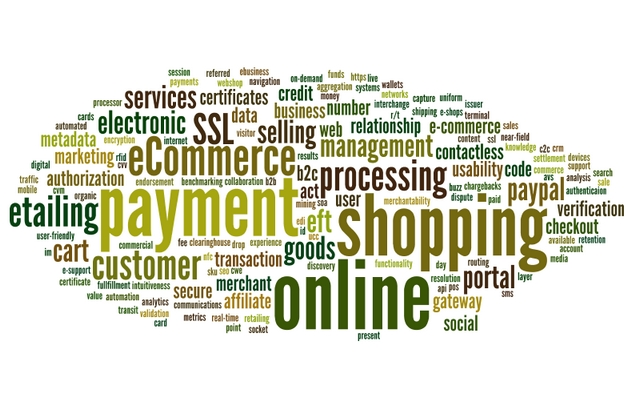
\includegraphics[width=0.8\linewidth]{images/introduction/ecommerce-wordle.jpg}\hfill
 \caption[e-commerce wordle]{e-commerce wordle}
 \label{fig:e_commerce_wordle}
\end{figure}
The strong competition and speed that characterize on-line market
accentuate the importants of the “time to market” that is the rapidity or speed with which a company manages to get the products reach the customer end.
\newline
Gradually there appeared many service providers to simplify and accelerate the process of creating and installing the e-commerce platforms.
\newline
Shopify, Bigcommerce, Prestashop, 3DCart, WIX.com are some of the best known and used platforms that offer services to insert, edit and delete products, manage inventory, create collections of products, putting one or more services available for payment, shipping / tracking, etc., all these through user-friendly interface so that anyone can use them.
\newline
In general, these services are well established and reliable.
But as the time has passed, these earlier technologies are now replaced by modern and viable substitutes.
\newline
The work presented in this thesis, carried out at the CVDLAB, consists of the high-level study of the main platforms for e-commerce that exist today, in order to identify an abstract data model capable of synthesizing the valuable features currently offered. Here,a new model is deployed, that is, X-commerce, using modern technologies such as Polymer, Loopback and NodeJS.
\newline
X-commerce uses pervasively the Polymer technology, which implements the standards of the Web Components, whose main feature is the reusability of code. As stated by the authors of Polymer-Project: “Everything is an element” \cite{polymer_world_view}. This is the philosophy that X-commerce follows, so any type of function or responsibility is encapsulated in different and self-contained elements of Polymer. Therefore X-commerce has an objective to highlight and project the concept of the Web Components up to the realization of a large-scale platform, that is, e-commerce.
\newline
X-commerce aims to provide developers with a new method, based on reusable components, to compose their own web pages (oriented to e-commerce). So, the creation of a web page is done by utilizing these varied reusable elements.
\newline
The thesis is divided into two parts: The first deals with the history of the e-commerce platform, the indispensable services for e-commerce systems and technologies used. The second part examines in detail the x-commerce project in its entirety. In particular, the first chapter of part one describes on the platforms that facilitate the realization of e-commerce systems like Shopify, Bigcommerce, Prestashop, etc. The second chapter describes the key enablers for payment services providers, and the third shows a general overview of the main technologies used to create X-commerce as Polymer, Loopback, etc.
\newline
The fourth chapter describes the architecture of X-commerce highlighting the main patterns and its models.
The fifth chapter focuses primarily on the management of payments, a service essential for an e-commerce system; while the sixth chapter and the general conclusions drawn exposes and provides the possiblity for future development of the project.